\chapter{Исследовательская часть}

\section{Технические характеристики}

Технические характеристики устройства, на котором выполнялись замеры по времени:

\begin{itemize}
    \item Процессор: Intel i5-1035G1 (8) @ 3.600 ГГц.
    \item Оперативная память: 16 ГБайт.
    \item Операционная система: Manjaro Linux x86\_64 (версия ядра Linux 5.15.131-1-MANJARO).
\end{itemize}

Во время проведения измерений времени ноутбук был подключен к сети электропитания и был нагружен только системными приложениями.

\section{Демонстрация работы программы}

На рисунке \ref{fig:prog-demo} показан пример работы разработанной программы для случая, когда пользователь выбирает действие <<Запуск алгоритмов поиска расстояния Левенштейна>> и вводит строки <<кошка>> и <<броненосец>>.

\clearpage
\begin{figure}[h]
    \centering
    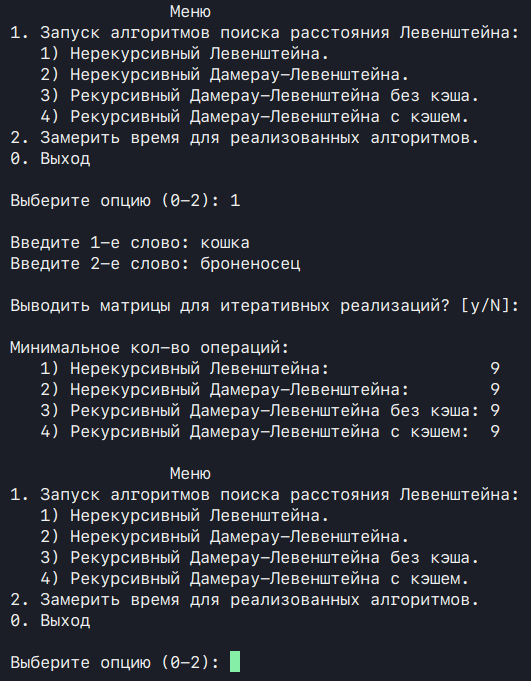
\includegraphics[height=0.6\textheight]{images/prog_demo.png}
    \caption{Демонстрация работы программы}
    \label{fig:prog-demo}
\end{figure}

\section{Временные характеристики}

Исследование временных характеристик реализованных алгоритмов производилось на строках длинами:

\begin{itemize}
    \item 1 -- 10 c шагом 1 для всех реализаций;
    \item 10 -- 200 c шагом 25 только для нерекурсивных реализаций.
\end{itemize}

В силу того, что время работы алгоритмов может колебаться в связи с различными процессами, происходящими в системе, для обеспечения более точных результатов измерения для каждого алгоритма повторялись 500 раз, а затем бралось их среднее арифметическое значение.

На рисунке \ref{fig:nonrec-time} показаны зависимости времени выполнения матричных реализаций алгоритмов Левенштейна и Дамерау~---~Левенштейна от длин входящих строк.

На рисунке \ref{fig:rec-time} показаны зависимости времени выполнения рекурсивных реализаций алгоритмов Левенштейна и Дамерау~---~Левенштейна от длин входящих строк.

На рисунке \ref{fig:dl-all-time} показаны зависимости времени выполнения рекурсивных реализаций алгоритма Дамерау~---~Левенштейна от длин входящих строк.

\begin{figure}[H]
    \centering
    \includesvg[width=1.0\textwidth]{images/nonrec.svg}
    \caption{Результат измерений времени работы нерекурсивных реализаций алгоритмов поиска расстояний Левенштейна и Дамерау~---~Левенштейна}
    \label{fig:nonrec-time}
\end{figure}

\begin{figure}[H]
    \centering
    \includesvg[width=1.0\textwidth]{images/rec.svg}
    \caption{Результат измерений времени работы рекурсивных реализаций алгоритма поиска расстояния Дамерау~---~Левенштейна}
    \label{fig:rec-time}
\end{figure}

\begin{figure}[H]
    \centering
    \includesvg[width=1.0\textwidth]{images/dl_all.svg}
    \caption{Результат измерений времени работы реализаций алгоритмов поиска расстояния Дамерау~---~Левенштейна}
    \label{fig:dl-all-time}
\end{figure}

\section{Характеристики по памяти}

Введем следующие обозначения:

\begin{itemize}
    \item $m$~--- длина строки $S_1$;
    \item $n$~--- длина строки $S_2$;
    \item $\text{size}(v)$~--- функция, вычисляющая размер входного параметра $v$ в байтах;
    \item $char$~--- тип данных, используемый для хранения символа строки;
    \item $int$~--- целочисленный тип данных.
\end{itemize}

Теоретически оценим объем используемой памяти итеративной реализацией алгоритма поиска расстояния Левенштейна:

\begin{multline}
    M_{LevIter} = (m + 1) \cdot (n + 1) \cdot \text{size}(int) + (m + n) \cdot \text{size}(char) + \\
    + \text{size}(int**) + (m + 1) \cdot \text{size}(int*) + \\
    + 3 \cdot \text{size}(int) + 2 \cdot \text{size}(int)
\end{multline}
где $(m + 1) \cdot (n + 1) \cdot \text{size}(int)$~--- размер матрицы,
\newline $\text{size}(int**)$~--- размер указателя на матрицу,
\newline $(m + 1) \cdot \text{size}(int*)$~--- размер указателей на строки матрицы,
\newline $(m + n) \cdot \text{size}(char)$~--- размер двух входных строк,
\newline $2 \cdot \text{size}(int)$~--- размер переменных, хранящих длину строк,
\newline $3 \cdot \text{size}(int)$~--- размер дополнительных переменных.

Для алгоритма поиска расстояния Дамерау~---~Левенштейна теоретическая оценка объема используемой памяти идентична.

Произведем оценку затрат по памяти для рекурсивных реализаций алгоритма нахождения расстояния Дамерау~---~Левенштейна.

Сперва рассчитаем объем памяти, используемой каждым вызовом функции поиска расстояния Дамерау~---~Левенштейна:
\begin{equation}
    M_{call} = (m + n) \cdot \text{size}(char) + 2 \cdot \text{size}(int) + 3 \cdot \text{size}(int) + 8
\end{equation}
где $(m + n) \cdot \text{size}(char)$~--- объем памяти, используемый для хранения двух строк,
\newline $2 \cdot \text{size}(int)$~--- размер двух входных строк,
\newline $3 \cdot \text{size}(int)$~--- размер дополнительных переменных,
\newline 8 байт~--- адрес возврата.

Максимальная глубина стека вызовов при рекурсивной реализации равна сумме длин входящих строк, поэтому максимальный расход памяти равен

\begin{equation}
    M_{DLRec} = (m + n) \cdot M_{call}
\end{equation}
где $m + n$~--- максимальная глубина стека вызовов,
\newline $M_{call}$~--- затраты по памяти для одного рекурсивного вызова.

Рекурсивная реализация алгоритма поиска расстояния Дамерау~---~Левенштейна с кэшированием для хранения промежуточных значений использует матрицу (кэш), размер которой можно рассчитать следующим образом:

\begin{multline}
	M_{cache} = (n + 1) \cdot (m + 1) \cdot \text{size}(int) +\\+ \text{size}(int **) + (m + 1) \cdot \text{size}(int *)
\end{multline}
где $(n + 1) \cdot (m + 1)$~--- количество элементов в кэше,
\newline $\text{size}(int **)$~--- размер указателя на матрицу,
\newline $(m + 1) \cdot \text{size}(int *)$~--- размер указателя на строки матрицы.

Таким образом, затраты по памяти для рекурсивного алгоритма нахождения расстояния Дамерау~---~Левенштейна с использованием кэша:

\begin{equation}
    M_{DLRecCache} = M_{DLRec} + M_{cache}
\end{equation}

\section{Вывод}

В результате исследования реализуемых алгоритмов по времени выполнения можно сделать следующие выводы:

\begin{enumerate}
    \item При небольших длинах строк (длина < 5 симв.) разница между временем выполнения нерекурсивных реализаций алгоритмов Левенштейна и Дамерау~---~Левенштейна незначительна.
    Однако, при увеличении длины обрабатываемых строк алгоритм поиска расстояния Дамерау~---~Левенштейна выполняется на порядок дольше, что связано с обработкой дополнительного условия о перестановке символов (см. рис. \ref{fig:nonrec-time}).
    \item Рекурсивная реализация алгоритма поиска расстояния Дамерау~---~Левенштейна с использованием кэша работает на порядок быстрее реализации поиска этого расстояния без кэширования (см. рис. \ref{fig:rec-time}).
    \item Время работы матричной и рекурсивной с кэшем реализаций алгоритма поиска расстояния Дамерау~---~Левенштейна приблизительно равны и выполняются на порядок быстрее в сравнении с рекурсивной реализацией поиска этого расстояния без кэширования (см. рис. \ref{fig:dl-all-time}).
\end{enumerate}

В результате исследования алгоритмов по затрачиваемой памяти можно сделать вывод о том, что итеративные алгоритмы и рекурсивный алгоритм с кэшированием требуют больше памяти по сравнению с рекурсивным без оптимизаций.
В реализациях, использующих матрицу, максимальный размер используемой памяти увеличивается пропорционально произведению длин строк, в то время как у рекурсивного алгоритма без кэширования объем затрачиваемой памяти увеличивается пропорционально сумме длин строк.